% TeX шаблон, пример оформления отчёта по лабораторной работе.
% Автор: Шмаков И.А.
% Версия от: 05 ноября 2018 года.
% Сборка документа из командной строки:
% ~$ pdflatex -shell-escape main.tex

\documentclass[a4paper,14pt]{extarticle}
\usepackage[utf8]{inputenc}
\usepackage[T2A]{fontenc}
\usepackage[english,russian]{babel}

% одинарный интервал
\usepackage{setspace}
\singlespacing 

\usepackage[left=3cm, right=1cm, top=1.5cm, bottom=1.5cm]{geometry}
\usepackage{icomma} % "Умная" запятая: $0,2$ --- число, $0, 2$ --- перечисление
\usepackage{indentfirst} % Красная строка.

% для гиперссылок и выделение их цветом
\usepackage{xcolor}
\usepackage{hyperref}

 % Цвета для гиперссылок
\definecolor{linkcolor}{HTML}{000000} % цвет ссылок
\definecolor{urlcolor}{HTML}{799B03} % цвет гиперссылок
\hypersetup{pdfstartview=FitH,  linkcolor=linkcolor, urlcolor=urlcolor, colorlinks=true}

% Пакет отвечающий за листинги.
\usepackage[outputdir=build]{minted} 
\renewcommand\listingscaption{Листин}

% Фикс "red box" в minted 
\usemintedstyle{xcode}

% Подключение графики
\usepackage{graphicx}
\usepackage{float}
\DeclareGraphicsExtensions{.png}

\renewcommand{\thesection}{\arabic{section}}

\begin{document}
\begin{titlepage}
  \begin{center}
    \MakeUppercase{Министерство науки и высшего образования Российской Федерации} \\
    \MakeUppercase{ФГБОУ ВО Алтайский государственный университет}
    \vspace{0.25cm}
    
    Физико-технический факультет
    
    Кафедра вычислительной техники и электроники
    \vfill
    
    \textsc{Отчёт по лабораторной работе №0 по курсу \\ <<Практикум по ТРПО>>}
  \bigskip

\end{center}
\vfill

\newlength{\ML}
\settowidth{\ML}{«\underline{\hspace{0.6cm}}» \underline{\hspace{2cm}}}
\hfill\begin{minipage}{0.5\textwidth}
  Выполнил студент 4-го курса, \\ 576 группы:\\
  \underline{\hspace{\ML}} В.\,Е.~Щербаков\\
  «\underline{\hspace{0.7cm}}» \underline{\hspace{2cm}} \the\year~г.
\end{minipage}%
\bigskip

\settowidth{\ML}{«\underline{\hspace{0.6cm}}» \underline{\hspace{2cm}}}
\hfill\begin{minipage}{0.5\textwidth}
  Проверил\\
  \underline{\hspace{\ML}} П.\,Н.~Уланов\\
  «\underline{\hspace{0.7cm}}» \underline{\hspace{2cm}} \the\year~г.
\end{minipage}%
\vfill

\begin{center}
  Барнаул, \the\year~г.
\end{center}
\end{titlepage}

\tableofcontents

\newpage

\section{Введение и постановка задачи}
В данной лабораторной работе необходимо реализовать программу с GUI для перемножения двух матриц:

$C[i][j] = \sum\limits_{i=0}^{k - 1} A[i][l]B[l][j]; i \in [0, n - 1]; j \in [0, m - 1]. $ 

Размеры матриц А и B обозначаются буквами $n, k$ и $k, m$ соответственно, которые вводятся пользователям с помощью GUI. 

Так же должна присутствовать возможность экспорта матриц в формат \textbf{CSV}. 

Для полученной программы необходимо составить описание алгоритма программы, выбрать ПО для рисования блок-схемы.

\section{Теоретическое описание задачи}
Саму программа будет написана на языке \textbf{Python}, для отрисовки GUI используем библиотеку \textbf{PyQT5} в связи с наличием опыта работы с ней, перемножение матриц же будет выполнять с помощью библиотеки \textbf{Numpy}.

На данный момент существует несколько вариантов для оформления отчетов - пакет \textbf{MS Word}, система компьютерной верстки \textbf{TeX} и её различные макрорасширения. Все вышеперечисленной имеет в своем арсенале все необходимое для написания отчета - текстовый редактор, различные расширения для рисования, редактор математических формул.

Поскольку мною используется операционная система \textbf{GNU/Linux}, которая является не поддерживаемой со стороны ПО MS Word, так же ввиду больших неудобств связанных с MS Word (отсутствие возможности версионирования документов, неудобство ПО, etc..), я предпочитаю использовать системe компьютерной верстки TeX вместе с набором макрорасширений \textbf{LaTeX}.

В связи с требованиям к блок-схемам в отчете (использование векторной графики), для оформления блок-схем я буду использовать ПО \textbf{Inkscape}.

На территории Российской Федерации действует единая система программной документации (ЕСПД), частью которой является 
\href{http://docs.cntd.ru/document/9041994}{ГОСТ 19.701-90 <<Схемы алгоритмов программ, данных и систем>>}, 
поэтому для оформления блок-схемы требуется использовать правила, 
описанные в указанной системе.

Краткое описание требований:
\begin{enumerate}
	\item Схемы алгоритмов, программ, данных и систем (далее - схемы) 
	состоят из имеющих заданное значение символов, 
	краткого пояснительного текста и соединяющих линий.
	\item Схемы могут использоваться на различных уровнях детализации, 
	причем число уровней зависит от размеров и сложности задачи обработки данных. 
	Уровень детализации должен быть таким, чтобы различные части и 
	взаимосвязь между ними были понятны в целом.
	\item Схемы данных отображают путь данных при решении задач и определяют этапы обработки, 
	а также различные применяемые носители данных.
\end{enumerate}

\section{Алгоритм и блок-схема}
Алгоритм работы программы:

\begin{enumerate}
	\item Начало работы программы
	\item Инициализация графического интерфейса
	\item Ожидание и чтение ввода пользователя
	\item Если введенные значения не являются числами, то вывод окна с ошибкой 
		и переход к пункту \ref{exit}
	\item Заполнение двух матриц случайными значениями
	\item Умножение двух матриц друг на друга
	\item Проверка наличия папки для файлов с выгрузкой, 
	если папка существует, то переход к пункту \ref{after_papka_creation}
	\item Создание папки для файлов
	\item Запись первой матрицы в файл \label{after_papka_creation}
	\item Запись второй матрицы в файл
	\item Запись результирующей матрицей в файл
	\item Конец работы программы \label{exit}
\end{enumerate}

Блок-схема программы:
\begin{figure}
	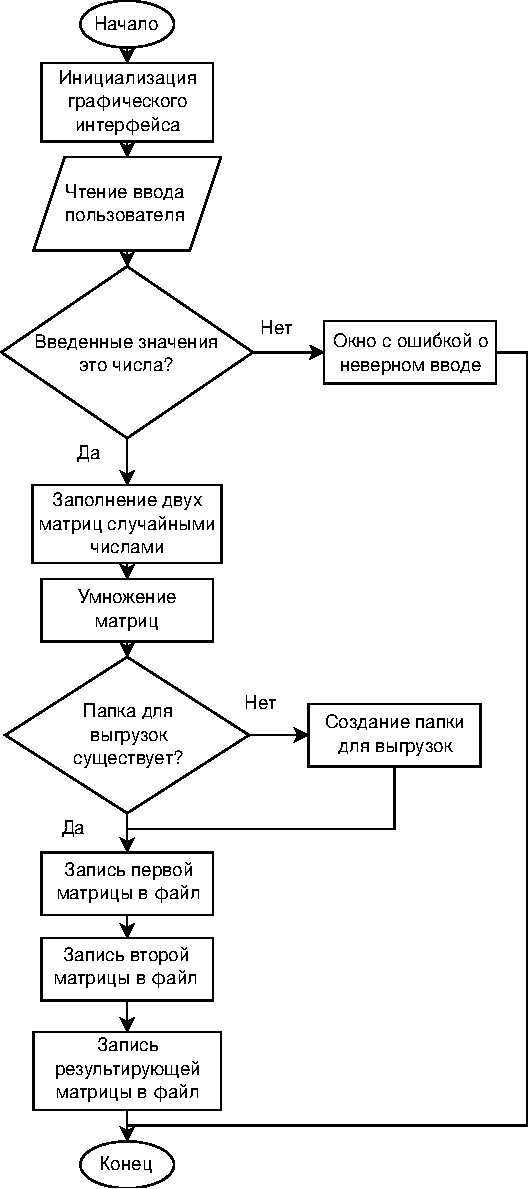
\includegraphics[width=\textwidth]{include/exported_diag.pdf}
	\caption{Блок-схема программы}
\end{figure}

\section{Проверка работы программы}
Для проверки работоспособности программы запустим её со следующими параметрами - 
$n = 2, k = 3, m = 2$.

В результате работы программы получим три файла:

Первая случайно сгенерированная матрица:
% minted не поддерживает csv, поэтому python
% Ах да, если убрать python - то все сломается :)
\begin{minted}[mathescape,linenos,breaklines]{python}
25,41,29
85,84,61
\end{minted}

Вторая случайно сгенерированная матрица:
\begin{minted}[mathescape,linenos,breaklines]{python}
7,71
91,1
33,73
\end{minted}

Результат умножения двух матриц:
\begin{minted}[mathescape,linenos,breaklines]{python}
4863,3933
10252,10572
\end{minted}

\newpage

\addcontentsline{toc}{section}{Выводы по работе}
\section*{Выводы по работе}
В ходе выполнения лабораторной работы были освежены знания языка Python и библиотеки PyQt5, были получены навыки использования библиотеки Numpy.

Данный отчет оформлен в среде LaTeX, которая обладает большой гибкостью и расширяемостью за счет подключаемых модулей, но при этом является довольно трудоемкой в плане освоения, так как некоторые вещи делаются очень нетривиальным образом и необходимо знать синтаксис системы LaTeX.

\newpage

\addcontentsline{toc}{section}{Приложение}
\section*{Приложение}
\inputminted[mathescape,linenos,breaklines]{python}{../src/main.py}

\end{document}          
